\documentclass[12pt]{article}
\usepackage{amsmath}
\usepackage{amsthm}
\usepackage{amsfonts}
\usepackage{graphicx}
\usepackage{epstopdf}
\usepackage{float}
\usepackage{fancyhdr}
\usepackage{hyperref}
\usepackage{subcaption}
\usepackage{pdfpages}
\usepackage{algpseudocode}
\usepackage{framed}
\usepackage{amssymb}



\makeatletter
\renewcommand\@biblabel[1]{}
\renewenvironment{thebibliography}[1]
     {\section*{\refname}%
      \@mkboth{\MakeUppercase\refname}{\MakeUppercase\refname}%
      \list{}%
           {\leftmargin0pt
            \@openbib@code
            \usecounter{enumiv}}%
      \sloppy
      \clubpenalty4000
      \@clubpenalty \clubpenalty
      \widowpenalty4000%
      \sfcode`\.\@m}
     {\def\@noitemerr
       {\@latex@warning{Empty `thebibliography' environment}}%
      \endlist}
\makeatother

\theoremstyle{definition}
\allowdisplaybreaks
\fancyhf{}


\DeclareMathOperator*{\Max}{Max}
\DeclareMathOperator*{\Min}{Min}
\setlength{\parindent}{0cm}



\begin{document}

\title{Endogenous long-run output impacts of monetary and fiscal policy: a growth theory approach}
\date{}
\author{Daniel H. Stahl}

\maketitle

\newpage
 \begin{abstract}

Traditional economic growth models do not include the impact of government policy on long-run growth.  Conversely, macro-models are often focused on the short-term impacts of government policy in closing an ``output gap'' and don't model the possible long term impacts of government policy on economic output.  In this paper I propose that both monetary and fiscal policy can have long-term impacts on economic growth.  Lower interest rates induce investment in riskier and more entrepreneurial endeavors.  This also causes a shift in labor towards entrepreneurial endeavors.  This pool of labor impacts the technological advances which improve the remaining labor's productivity.  Fiscal policy impacts long run growth reducing the economy's effective labor.  This occurs for two reasons: first, the expanded bureaucratic state requires labor to administer.  While this may be a small number relative to the total population, it may have an outsized impact on highly skilled labor.  Second, fiscal policy may dis-incentivize labor participation at the margins, thus reducing output.  I find that, in this model, high rates of interest reduce technological innovation which constrains output per capita to a constant long-run level.  ``Normal'' levels of government spending have mild impacts on output, while high levels may cause output to crash to zero as enough labor is dis-incentived from work.   
\\
\\
Core Results:
\begin{enumerate}
\item Long run growth model incorporates

\end{enumerate}

Keywords: 
\end{abstract}


\newpage
\section{Introduction}

Traditional economic growth models do not include the impact of government policy on long-run growth \cite{solow}. Conversely, macro-models are often focused on the short-term impacts of government policy in closing an ``output gap'' and don't model the possible long term impacts of government policy on economic output \cite{mankiwreis}.  In this paper I propose that both monetary and fiscal policy can have long-term impacts on economic growth.  Lower interest rates induce investment in riskier and more entrepreneurial endeavors.  This also causes a shift in labor towards entrepreneurial endeavors.  This pool of labor impacts the technological advances which improve the remaining labor's productivity.  Fiscal policy impacts long run growth reducing the economy's effective labor.  This occurs for two reasons: first, the expanded bureaucratic state requires labor to administer.  While this may be a small number relative to the total population, it may have an outsized impact on highly skilled labor.  Second, fiscal policy may dis-incentivize labor participation at the margins, thus reducing output.  I use an enhanced Solow-style model with a Cobb-Douglas production function which includes monetary and fiscal policy impacts.

\section{Model}

\subsection{Definitions}
There are three homogenous pools of labor.  \(L_1(t)\) is labor that, combined with capital, produces output.  \(L_2(t)\) is labor that works in research and development.  This labor creates technological efficiencies, \(A(t)\), which enhance the productivity of \(L_1(t)\).  Finally, there is \(L_3(t)\), which is either the ``bureaucratic'' labor which maintains the administrative state, or represents capable labor that chooses not to participate in the labor force.  Since \(L_3(t)\) does not impact the output, the model is agnostic to whether labor force participation or bureaucratic administration is the primary driver of \(L_3(t)\).  There is capital \(K(t)\).  \(i\) is the interest rate set by the central bank, which is assumed to be exogenously shocked and then reverts to the natural rate.  \(g\) is the fraction of output that is used for government spending.  It is assumed that this spending is neutral from an output perspective: that is, labor and capital that is employed through fiscal policy has the same output as private sector labor and capital and in the same proportions.
\\
\\
Following Solow \cite{solow}, output \(Y(t)\) takes the following form:

\[Y(t)=K(t)^\alpha (A(t)L(t)V_3(t))^{1-\alpha}\]

\(V_3(t)\) is the fraction of total labor that is performing traditional labor; as opposed to bureaucratic or research labor.  

\subsection{Dynamics}

Labor grows exponentially.

\[\frac{dL}{dt}=\eta L(t)\]

Defining \(i^*\) as the long run interest rate, \(i(s)\) as the current interest rate, \(g\) as the fraction of output from government spending, and 

\[l_1=e^{\gamma_0+\gamma_1 \int_0^t \left(i^*-i(s)\right) ds+\gamma_2 \int_0^t g(s) ds }\]
\[l_2=e^{\phi_0+\phi_1 \int_0^t g(s) ds}\]

Then the fractions of labor into the ``research'',  ``bureaucratic'', and ``traditional'', are governed by the following respectively:

\[V_1(t)=\frac{l_1(t)}{1+l_1(t)+l_2(t)}\]
\[V_2(t)=\frac{l_2(t)}{1+l_1(t)+l_2(t)}\]
\[V_3(t)=\frac{1}{1+l_1(t)+l_2(t)}\]

Where \(\gamma_0\) is the non-intervention (baseline) rate of growth in research labor, \(\gamma_1\) is the sensitivity of labor to the prevailing interest rate's deviation from the ``natural'' rate \(i^*\), and \(\gamma_2\) is the proportion of government spending that is dedicated to research and development.  For instance, federal grants to universities would be considered spending on basic research.  \(\phi_0\) is the (presumably small) administrative state in the case of zero government involvement in the economy, and \(\phi_1\) measures the growth of the administrative state as the government's involvement in the economy grows larger. 

The interest rate \(i\) has the following dynamics: 

\[\frac{di(t)}{dt}=a\left(i^*-i\right)\]

The government impact is ``sticky'' and impacts \(V_1\) and \(V_2\) at a rate \(b\).

\[\frac{dg(t)}{dt}=b\left(g^*-g\right)\]

Note that while monetary policy shocks \(i\) which then reverts at rate \(a\) to \(i^*\), the fiscal policy is assumed permanent and adjusts \(g^*\), with \(g(t)\) adjusting at rate \(b\) to the new permanent level.
\\
\\
Solving the integrals,
\[l_1=e^{\gamma_0+\gamma_1  \left(i^*-i(0)\right)e^{-a t}+\gamma_2 \left( g_0 e^{-b t}+g^*\left(1-e^{-b t}\right) \right) }\]
\[l_2=e^{\phi_0+\phi_1  \left( g_0 e^{-b t}+g^*\left(1-e^{-b t}\right) \right)}\]
\\
\\
Technology dynamics are directly proportional to the labor dedicated to research.  While in reality research requires some level of capital, the assumption simplifies the analysis.  Many kinds of research (for example, mathematics and economics) requires minimal capital investment.  Of course, the physical sciences often require massive capital investments.  This is a shortcoming of the model.  Note that this also deviates from the classic Solow model where technological growth is exogoneous.
\[\frac{dA(t)}{dt}=\beta L(t) V_1(t)\]

Finally, capital follows the familiar dynamics from Solow:
\[\frac{dK(t)}{dt}=s Y(t) - \delta K(t)-  L(t) V_1(t)\]
\(s\) is the saving rate, \(\delta\) is the rate of capital depreciation, and it is assumed that investment in technology (via \( L(t) V_1(t)\)) crowds out investment in capital.  

\subsection{Model analysis}

I focus on output per capita, \(\frac{Y(t)}{L(t)}\). There are three possible long-run states to the model.  First is exponential growth.  Exponential growth occurs if \(V_1(t)\), \(V_2(t)\), and \(V_3\) reach non-zero steady states and the drift of \(K\) remains positive.  The second is a steady state.  This occurs if \(V_1(t)\) shrinks to zero, causing \(A(t)\) to converge to a constant.  The third is economic collapse.  This occurs if \(V_1(t)\) and \(V_2(t)\) are too large; causing capital \(K\) to have negative drift. 

\subsubsection{Exponential growth}
Exponential growth occurs if  
\[\lim_{t \to \infty} s K(t)^\alpha (A(t)L(t)V_3(t))^{1-\alpha} > \lim_{t \to \infty} \delta K(t) +  L(t) V_1(t)\] 
and \(\lim_{t \to \infty} V_1(t) > 0 \).

\subsubsection{Steady state}
A steady state occurs if  
\[\lim_{t \to \infty} s K(t)^\alpha (A(t)L(t)V_3(t))^{1-\alpha} > \lim_{t \to \infty} \delta K(t) +  L(t) V_1(t)\] 
and \(\lim_{t \to \infty} V_1(t) =0\).

\subsubsection{Economic collapse}
Economic collapse occurs if 
\[\lim_{t \to \infty}s K(t)^\alpha (A(t)L(t)V_3(t))^{1-\alpha} < \lim_{t \to \infty} \delta K(t) +  L(t) V_1(t)\] 
This can occur if too much labor is invested in technology (ie, \(V_1(t)\) is ``too high'') or if there is too much labor that is either not working or maintaining the bureaucratic state (ie, \(V_3(t)\) is ``too low'').                                

\section{Results}

Since the model is a system of non-linear differential equations, the model must be solved numerically.  I show plots of an economy under different interest rate and fiscal policy regimes.  The full parameters for this economy:

\begin{center}
\begin{tabular}{ c c }
      Variable  & Value  \\ 
      \(\eta\) & 0.02 \\  
      \(\gamma_0\) & 0.004   \\  
      \(\gamma_1\) & 1.5   \\  
      \(\gamma_2\) & 0.005   \\ 
      \(v_0\) & 0.001  \\  
      \(v_1\) & 0.05  \\  
      \(a\) & 0.1  \\
      \(\beta\) & 0.03   \\  
      \(\alpha\) & 0.4   \\  
      \(\delta\) & 0.1   \\  
      \(s\) & 0.3   \\ 
      \(L_1(0)\) & 3.0   \\ 
      \(L_2(0)\) & 1.0  \\ 
      \(L_3(0)\) & 1.0   \\ 
      \(A(0)\) & 2.0  \\ 
      \(K(0)\) & 10.0   
\end{tabular}
\end{center}

Monetary policy in either direction can lead to low growth or collapse.  An increase in interest rates can lead to lower levels of technology improvement, which can slow economic growth.  A decrease in interest rates can lead to unsustainable growth in technology labor, leading to economic collapse.  Similarly, as fiscal policy gets larger, more of the productive economy is ``crowded out''.  At very high levels of government spending, the economy tends towards collapse as non-productive labor increases.     

\begin{minipage}[c]{0.8\linewidth}
\begin{framed}
\centering
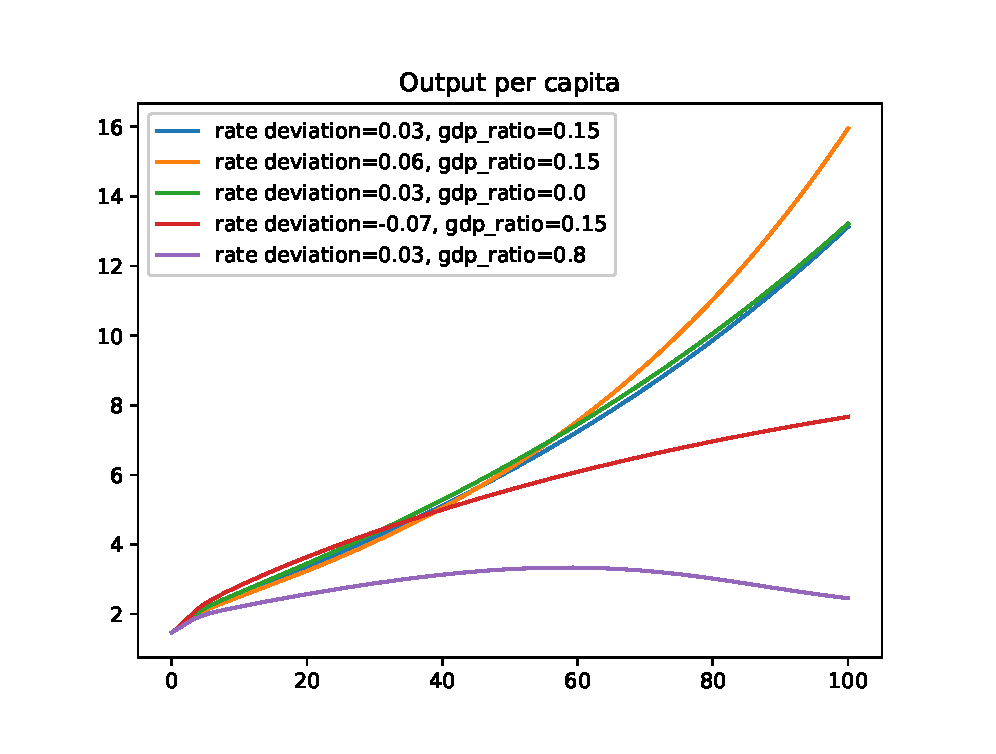
\includegraphics[width=1\textwidth]{images/economy_0}
\end{framed}
\end{minipage}


\begin{minipage}{\linewidth}
\begin{framed}
\begin{minipage}[t]{.48\textwidth}
\centering
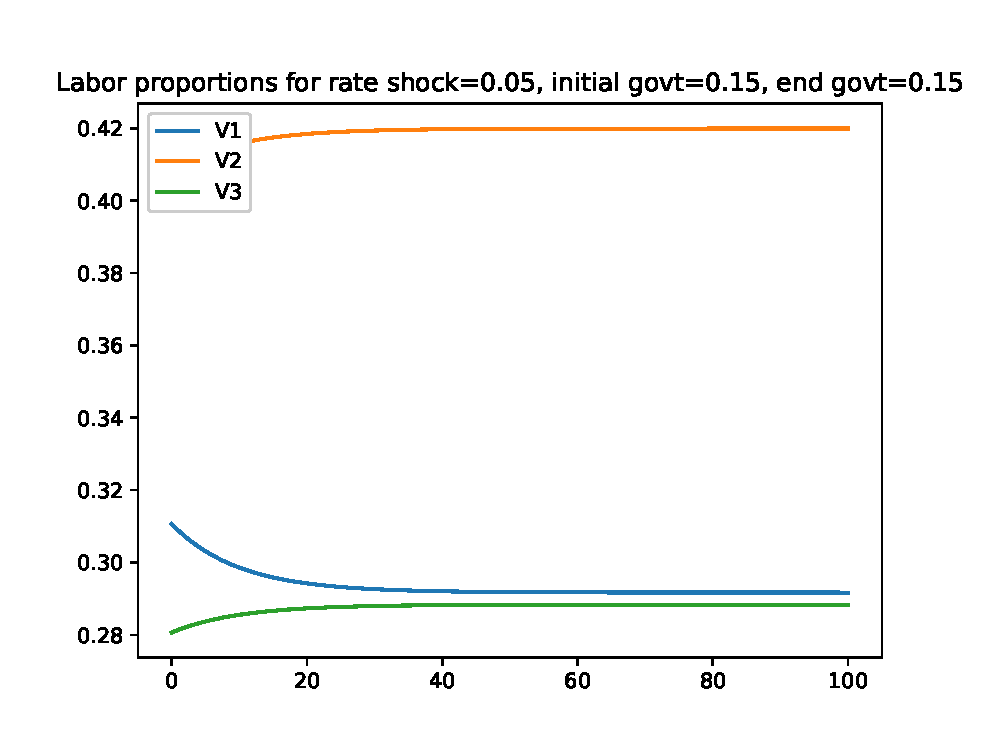
\includegraphics[width=1\textwidth]{images/econ_0_run_0_labor}
\end{minipage}\hfill
\begin{minipage}[t]{.48\textwidth}
\centering
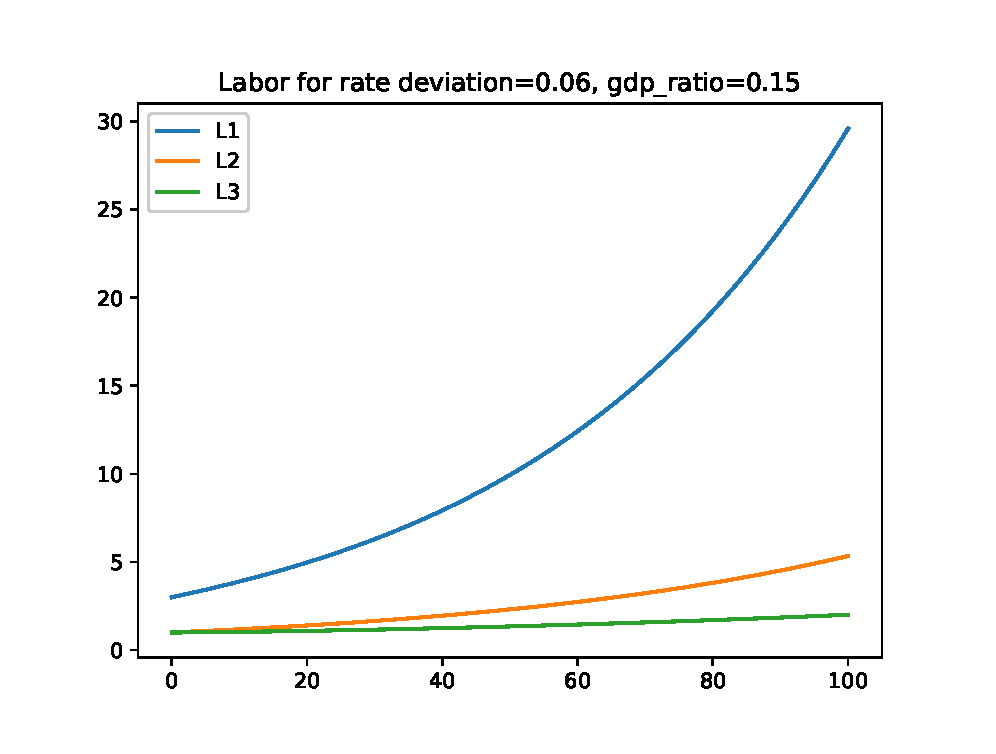
\includegraphics[width=1\textwidth]{images/econ_0_run_1_labor}
\end{minipage}\hfill
\begin{minipage}[t]{.48\textwidth}
\centering
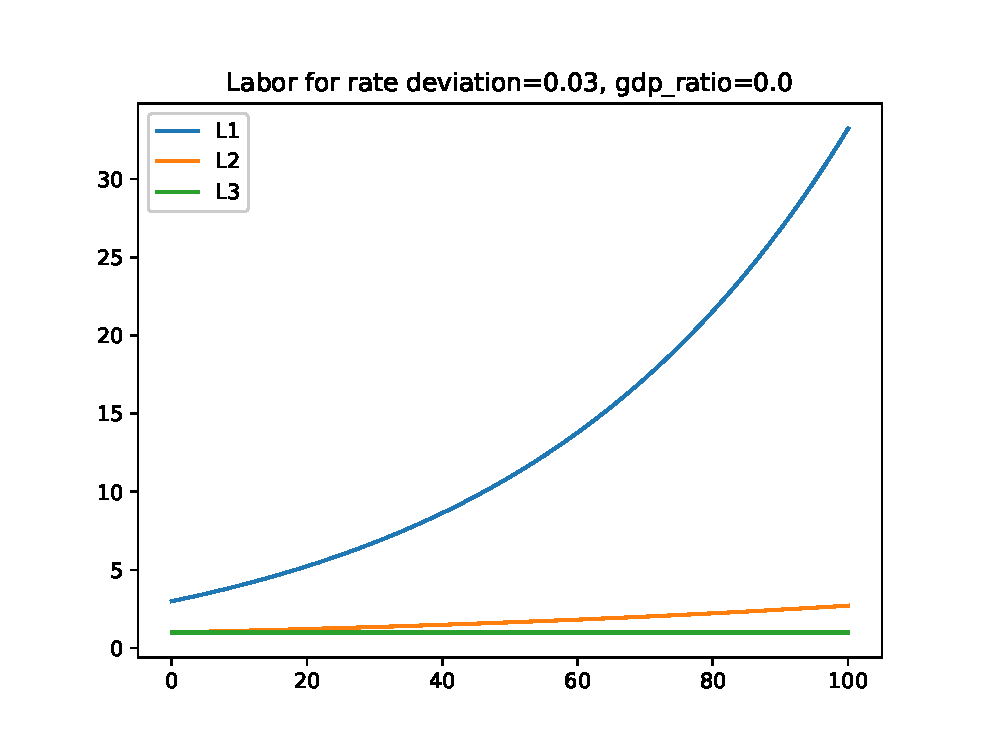
\includegraphics[width=1\textwidth]{images/econ_0_run_2_labor}
\end{minipage}\hfill
\begin{minipage}[t]{.48\textwidth}
\centering
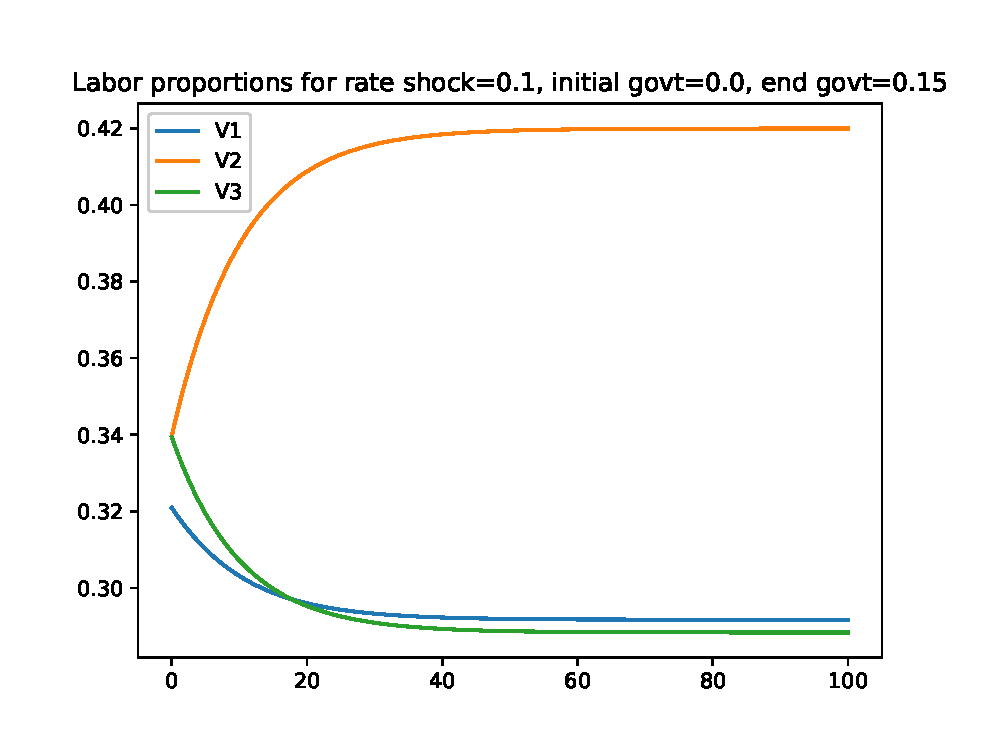
\includegraphics[width=1\textwidth]{images/econ_0_run_3_labor}
\end{minipage} \hfill
\begin{minipage}[t]{.48\textwidth}
\centering
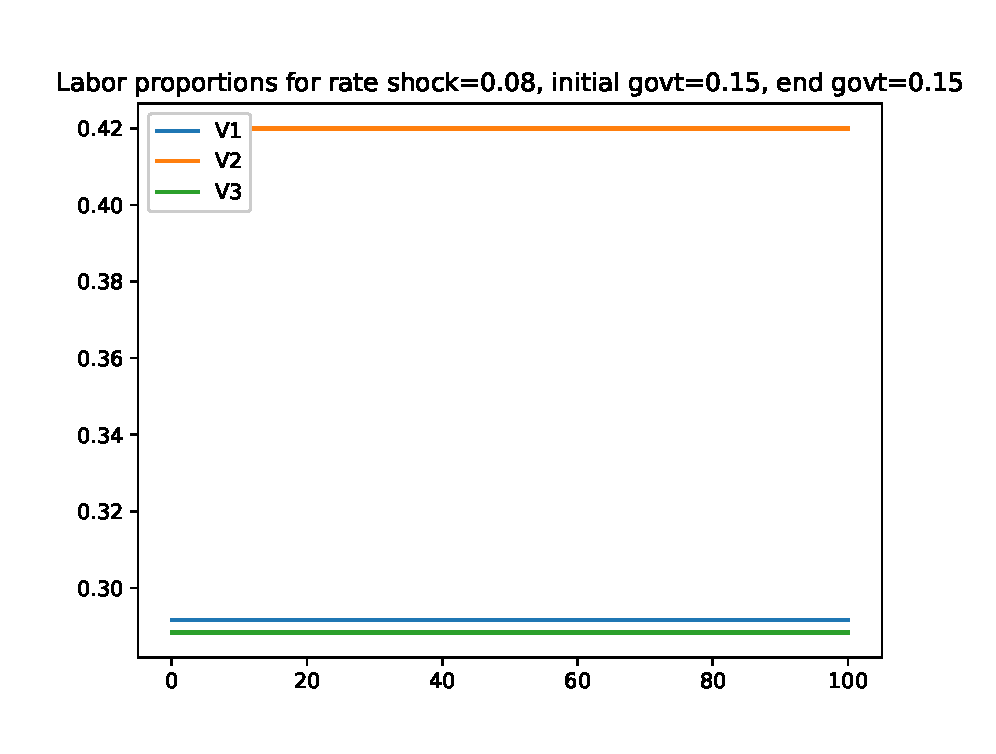
\includegraphics[width=1\textwidth]{images/econ_0_run_4_labor}
\end{minipage}\hfill
\begin{minipage}[t]{.48\textwidth}
\centering
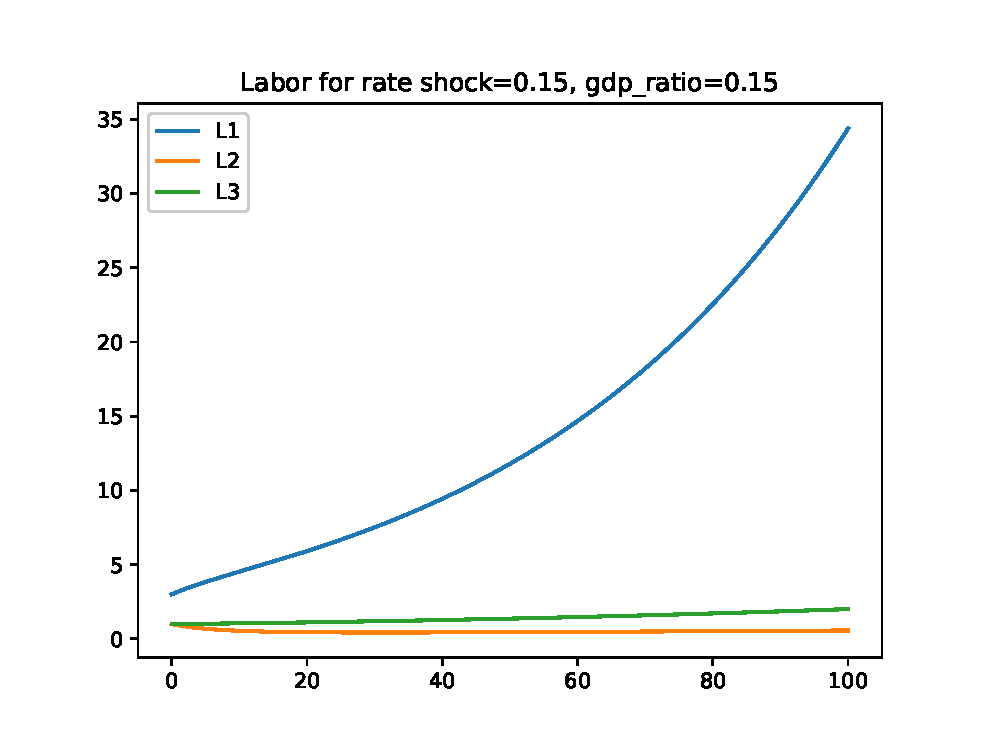
\includegraphics[width=1\textwidth]{images/econ_0_run_5_labor}
\end{minipage}\hfill
\begin{minipage}[t]{.48\textwidth}
\centering
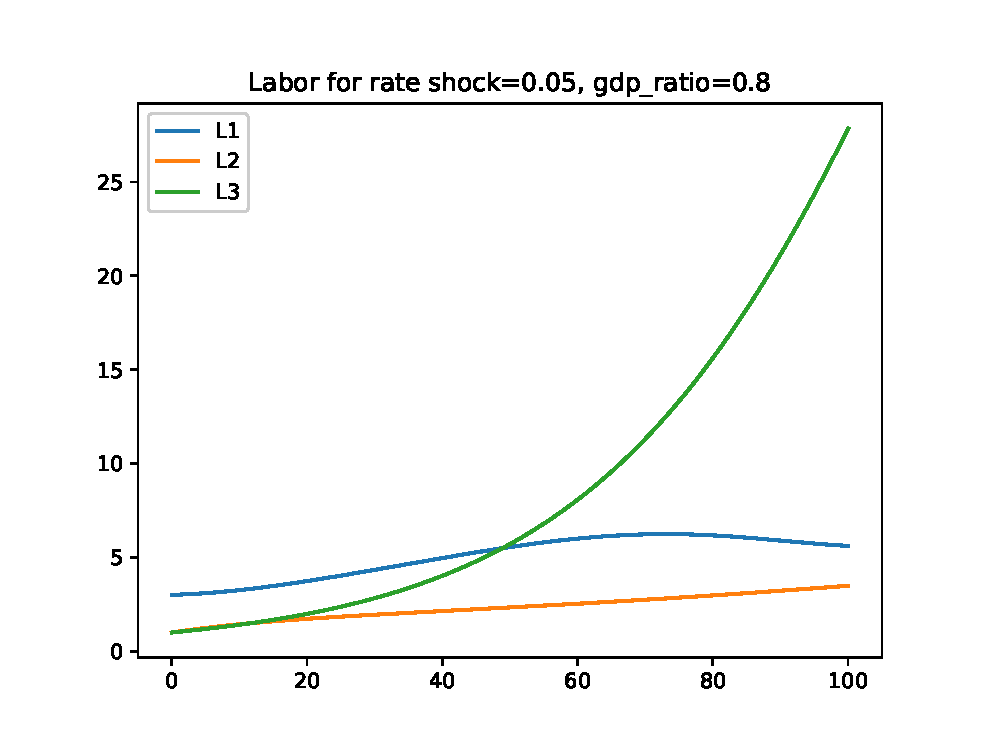
\includegraphics[width=1\textwidth]{images/econ_0_run_6_labor}
\end{minipage}\hfill
\end{framed}
\end{minipage}

The economy becomes stagnant when \(L_2\) goes to zero and collapses when \(L_3\) grows without bound.  For low levels of fiscal involvement there is a tradeoff between the positive impact that fiscal policy has on research and the disincentives to work and the increased size of the bureaucratic state.  As can be seen with the blue and green lines in the total output chart, the output difference between a 0\% and 15\% fiscal stimulus is very small.  It requires a quite large fiscal output (80\% of the economy) to lead to economic collapse.

\section{Conclusion}

This model introduced in this paper shows that fiscal and monetary policy can have long run impacts.  

\newpage
\begin{thebibliography}{9}
\bibitem{solow}
R Solow.  A Contribution to the Theory of Economic Growth.  \textit{The Quarterly Journal of Economics}, 70, (1), 1956.
\bibitem{mankiwreis}
N. Gregory Mankiw and Ricardo Reis.  Sticky Information Versus Sticky Prices: A Proposal To Replace The New Keynesian Phillips Curve. \textit{The Quarterly Journal of Economics} 117 (4), 2002.
\end{thebibliography}


\end{document}